\chapter{The Shared Annotator Setting}

%\label{sec:setting} 

In our setting, there are $K$  binary classification tasks to be learned simultaneously. 
In opposed to the common multi-task classification settings, here, no dependency between the tasks 
is assumed during the analysis, but the tasks can be dependent as well. 
The model learning is performed in rounds as an online learning algorithm, as following: 
On each round $t$, there are $K$ input-label pairs
$(\vxi{i,t},\yi{i,t})$, one for each classification task, where $i=1,2\comdots K$ is the task index and $t$ is the 
step index. The inputs $\vxi{i,t}\in\reals^{d_i}$ are vectors, and the labels  $\yi{i,t}\in\{-1,+1\}$ are binary. 
In the general case, the input-spaces for each problem may be different, and inputs may
have different number of elements. Yet, in order to  simplify the notation and without loss of generality,  
from now on, in our analysis we assume that for all of the tasks, $\vxi{i,t}\in\reals^{d}$. 
i.e. all the tasks are in the same dimension and $d_i = d$ holds for all tasks.
In practice, since the proposed algorithms use the margin that is affected by the vector norm, 
there is a need to scale all the vectors into a ball.

On round $t$, the learning algorithm receives $K$ input vectors $\vxi{i,t}$, 
for $i=1 \comdots K$ tasks and produce  $K$  binary-labels output $\hyi{i,t}$, where
$\hyi{i,t}\in\{-1,+1\}$ is the label predicted for the input
$\vxi{i,t}$ corresponds to the task $i$. The algorithm then chooses a task $J_t \in\
\{1 \comdots K\}$ and asks from an annotator its true-label. Unlike the usual online multi-task setting, and due to the limitation in our
case, it  does not observe any other label. 
Then, the algorithm updates its model, using the received feedback, and proceeds to the
next round and input examples.  
For the ease of the calculations below, we denote by $K$ indicators 
$Z_t=\paren{ Z_{1,t} \comdots Z_{K,t}}$, the identity of the task which was queried by the algorithm
on round $t$, and set $Z_{J_t,t}=1$  and $Z_{i,t}=0$ for $i\ne J_t$. 
Clearly from the definition, the condition, $\sum_i{Z_{i,t}=1} ,\forall{i,t}$, always holds. 
In order to use it in the analysis below, we define the notation $\Expp{t-1}{x}$ as well, to be the
conditional expectation $\Exp{x \vert Z_{1},\ldots Z_{t-1}}$ given all previous choices of the tasks to be queried.


\begin{table}[htp]
\begin{center}
{\rowcolors{1}{green!80!yellow!50}{green!70!yellow!40}
\centering
\begin{tabular}{|c c c c c c|} \hline
 Step &	1 &	2 &	3 &	4 &	5 \\  \hline
 Task 1 &	Q      &	NQ &	Q &	NQ &	NQ \\ \hline
 Task 2 &	NQ   &	NQ &	Q &	NQ &	NQ \\ \hline
 Task 3 &	Q      &	 NQ &	Q &	NQ &	NQ \\ \hline
 Task 4 &	Q      &	Q &	NQ &	NQ &	Q \\ \hline
\end{tabular}
}
\end{center}
\caption{In selective sampling we focus on when to issue a query for a single task (a row).}
\label{tab:multitask_selective_sampling_example}
\end{table}

\begin{table}[htp]
\begin{center}
{\rowcolors{1}{green!80!yellow!50}{green!70!yellow!40}
\centering
\begin{tabular}{|c c c c c c|} \hline
 Step &	1 &	2 &	3 &	4 &	5 \\  \hline
 Task 1 &	Q &	  NQ &	NQ &	NQ &	NQ \\ \hline
 Task 2 &	NQ &	NQ &	Q &	Q &	NQ \\ \hline
 Task 3 &	NQ &	 NQ &	NQ &	NQ &	Q \\ \hline
 Task 4 &	NQ &	Q &	NQ &	NQ &	NQ \\ \hline
\end{tabular}
}
\end{center}
\label{tab:multitask_SHAMPO_example} 
\caption{ In the SHAMPO setting we focus on when to issue a query for a single step (a column).}
\end{table}


Schematic illustration of a single iteratidblp:conf/nipson of multi-task algorithms is shown in \figref{fig:ilustration}. 
The top panel shows the standard setting of online multi-task algorithms with a shared annotator, that 
labels all inputs, which are fed to the corresponding algorithms to update corresponding models. The
bottom panel shows the SHAMPO algorithm, which couples labeling
annotation and learning process, and synchronizes a single annotation
per round.  At most one task performs an update per round, the one
with the annotated input.

\begin{figure}
\begin{centering}
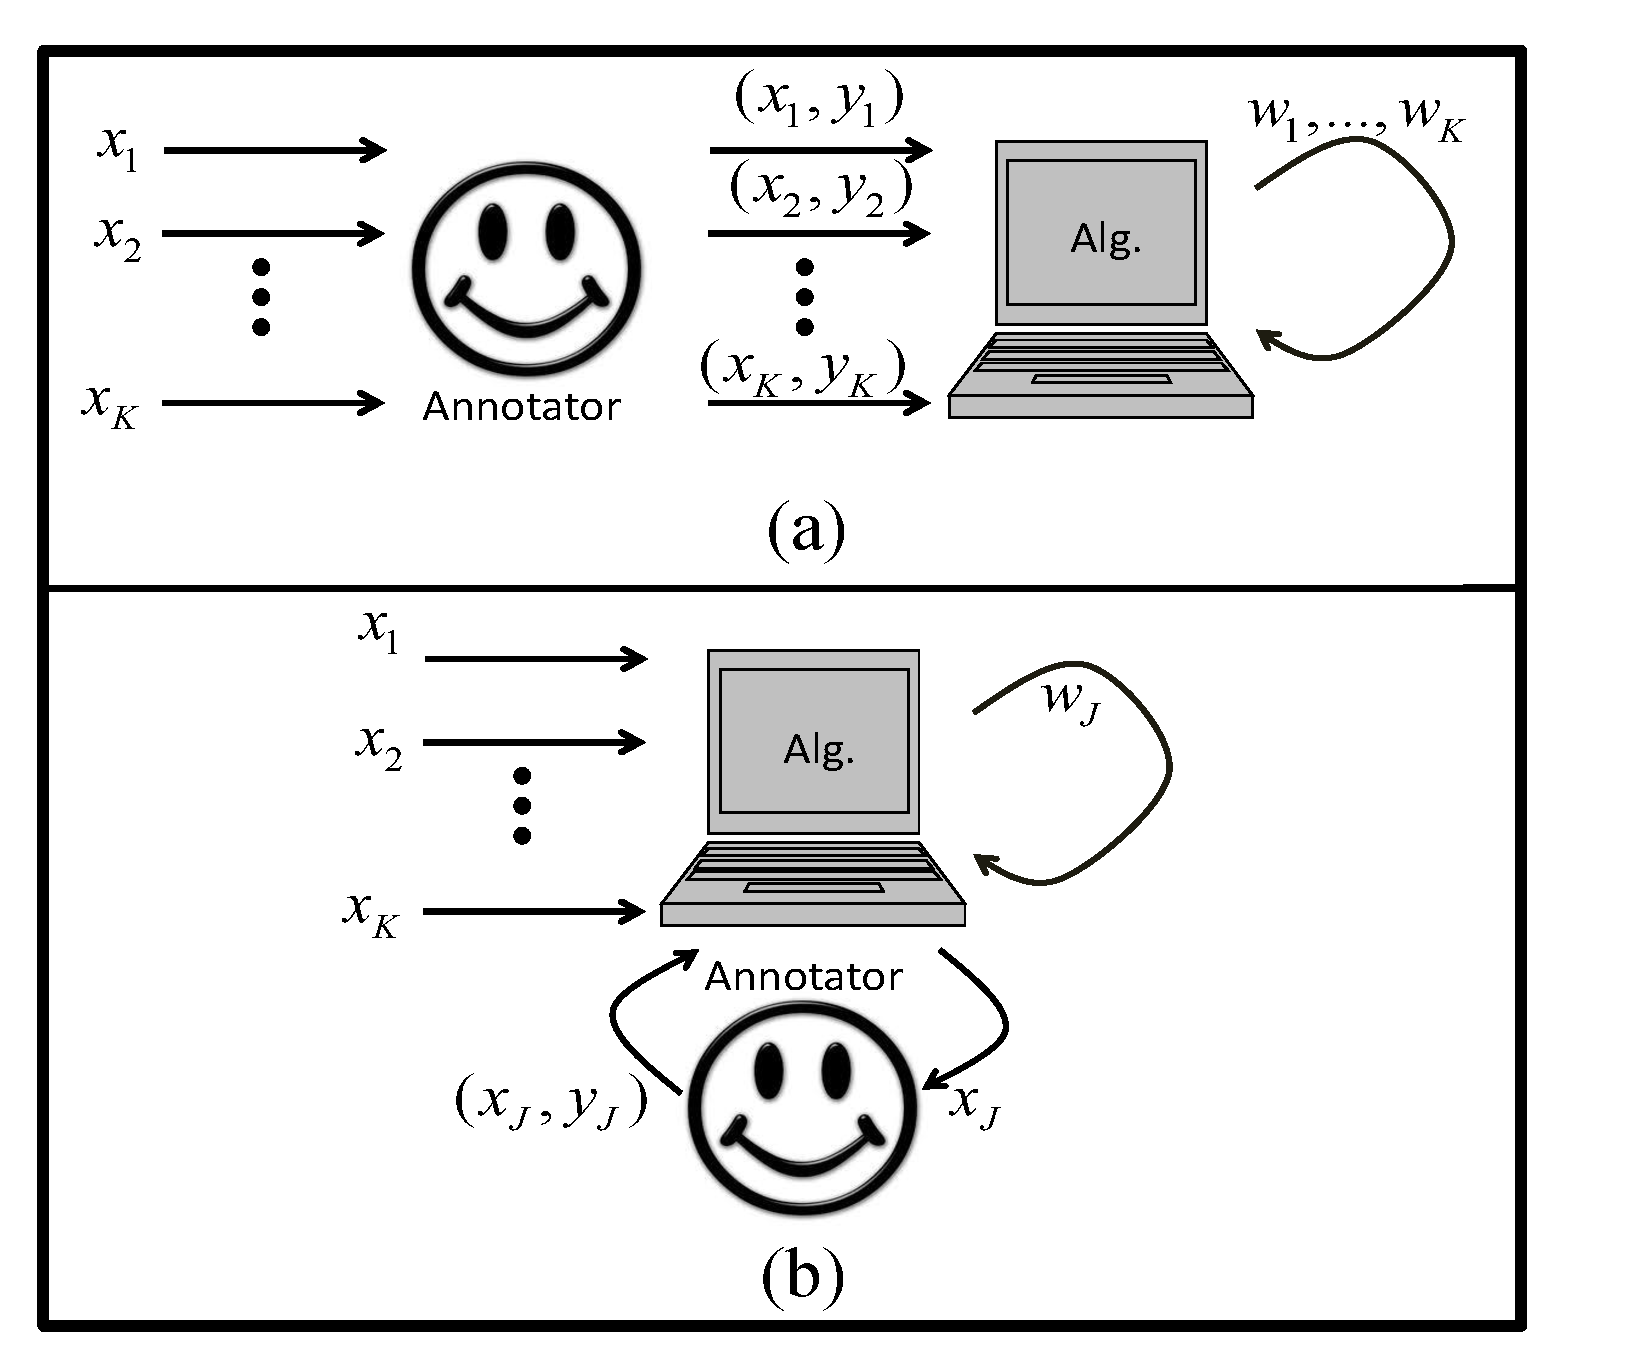
\includegraphics[width=0.5\textwidth]{figs/SHAMPO_illustration.eps}
\caption{Illustration of a single iteration of  multi-task algorithms: (a) standard setting and (b) SHAMPO setting}
\label{fig:ilustration}
\end{centering}
\end{figure}

As we have mentioned before, our setting is similar to the Selective Sampling 
case, in a sense that at every round we ask a single binary question. However, 
while the Selective Sampling algorithm asks ``when'' to issue a query, at each time step, our SAHMPO 
algorithm asks on ``which one'' of the tasks to issue a query. 
An example for the difference between the Selective Sampling multi-task problem and 
the SHAMPO setting is \tabref{tab:multitask_selective_sampling_example} and 
\tabref{tab:multitask_SHAMPO_example}. Where the cells are assigned with 'Q' (Queried) for tasks and 
rounds that the algorithm issue a query, and with 'NQ' (Not Queried) on tasks 
and rounds that the algorithm decided not to issue a query.
As a result of the setting difference, when we run multi-task problem as an independent Selective sampling 
tasks, we allow at each round, to query more than one query 
(e.g. \tabref{tab:multitask_selective_sampling_example} step 2), or even less than one query, i.e. 
not asking for a feedback at all (e.g. \tabref{tab:multitask_selective_sampling_example} step 4). 
The SHAMPO setting on the other hand, is more 
limited, since for every round, the algorithm  issue one, and only one query. 




